% This work is licensed under the Creative Commons Attribution-Share Alike 2.0 France.
% To view a copy of this license, visit http://creativecommons.org/licenses/by-sa/2.0/fr/legalcode.
% or send a letter to Creative Commons, 171 Second Street, Suite 300, San Francisco, California, 94105, USA


\chapter{8 multipliés par 3,57 égal...\label{chap:8}}
\section{Les calculs en Python}
Combien font 8 multipliés par 3,57? Vous pouvez utiliser une calculatrice, n'est-ce pas? 
Ou bien vous êtes peut-être extrêmement intelligent et vous pouvez faire la multiplication de tête mais ce n'est pas l'objet. 
Vous pouvez aussi faire la même chose avec la console Python.
Démarrez la console à nouveau (voir le chapitre 1 pour plus d'informations, si vous avez sauté le début pour quelque étrange raison) et une fois que vous voyez l'invite de commande, tapez \verb+8*3.57+ et appuyez sur entrée\footnote{Les anglo-saxons utilisent le point «~.~» comme séparateur décimal contrairement aux francophones.}.

\begin{Verbatim}[frame=single,rulecolor=\color{mbleu},label=à taper]
>>> 8*3.57
28.559999999999999
\end{Verbatim}

\setsansfont[Mapping=tex-text]{Linux Biolinum O}
L'étoile «~\verb+*+~», ou touche astérisque, est utilisée pour les multiplications,
à la place du symbole multiplier normal «~\textsf{x}~» que vous utilisez à l'école.
Utiliser la touche étoile est nécessaire, autrement comment les ordinateurs sauraient si vous voulez dire la lettre «~\emph{x}~» ou le symbole de multiplication «~\textsf{x}~»? Pour une équation n'est-ce pas légèrement utile?

\begin{center}

\fcolorbox{black}{lbleu}{
 \begin{minipage}{12cm}
\textbf{Python est cassé!}\\


Si vous avez juste pris une calculatrice et entré \texttt{8x3.57} la réponse qui devrait être affichée est la suivante: \texttt{28.56}.\\

Pourquoi Python est différent? Est-il cassé?\\

En fait non, la raison peut-être trouvée dans la manière dont les nombres à virgule flottante (nombres rationnels) sont gérés par l'ordinateur. Il s'agit d'un problème compliqué pour les débutants\footnote{Le problème provient du fait que l'ordinateur ne gère pas des fractions mais justement des nombres à virgules avec une quantité finie de chiffres.}. Le mieux, pour le moment, est juste de vous rappeler que lorsque vous travaillez avec des fractions (ou des nombres avec une virgule) quelques fois le résultat n'est pas précisément ce que vous attendiez. Cela est vrai pour les multiplications, les divisions, les additions et les soustractions\footnote{Il est bien sûr possible d'implémenter en Python des procédés semblables à ceux des calculatrices comme dans calculext: \url{http://python.jpvweb.com/mesrecettespython/calculext}.}.
\end{minipage}
 }
\end{center}



Supposons que vous faites le ménage une fois par semaine, pour cela vous recevez 5\begin{small}\euro\end{small} d'argent de poche, et vous livrez les journaux cinq fois par semaine et avez ainsi 30\begin{small}\euro\end{small} de plus par semaine. Combien gagnerez-vous par an ?

Si nous l'écrivons sur le papier, nous devront écrire quelque chose comme \texttt{(5\begin{small}\euro\end{small}+30\begin{small}\euro\end{small})x52} ce qui corresponde à 5\begin{small}\euro\end{small} plus 30\begin{small}\euro\end{small} multiplié par 52 semaines d'une année. Bien sûr nous sommes intelligents et nous savons que cinq plus trente font trente cinq et que l'équation se simplifie en \tt{}35\begin{small}\euro\end{small}x52\rm{} ce qui peut facilement être calculé à la main.

Mais nous pouvons faire tous ces calculs dans la console tout aussi bien:

\begin{Verbatim}[frame=single,rulecolor=\color{mbleu}, label=à taper]
>>> (5 + 30) * 52
1820
>>> 35 * 52
1820
\end{Verbatim}


Mais que ce passe-t-il si nous dépensons 10\begin{small}\euro\end{small} par semaine? Combien nous restera-t-il à la fin de l'année? Nous pouvons écrire l'équation à nouveau sur le papier quelques différentes manières, mais nous allons juste taper dans la console:

\begin{Verbatim}[frame=single,rulecolor=\color{mbleu}, label=à taper]
>>> (5 + 30 - 10) * 52
1300
\end{Verbatim}


Ce qui correspond à 5\begin{small}\euro\end{small} plus 30\begin{small}\euro\end{small} moins 10\begin{small}\euro\end{small} multipliés par les 52 semaines de l'année. Il vous reste ainsi 1300\begin{small}\euro\end{small} à la fin de l'année. Bon d'accord, ce que nous avons fait n'est pas si utile que cela jusqu'à maintenant. Nous pouvons faire tout cela avec une calculatrice. Mais nous y reviendrons plus tard et verrons comment rendre cela plus utile.

Vous pouvez faire des multiplications, des additions (évidemment), des soustractions et des divisions dans la console Python; ainsi qu'un tas d'autres opérations mathématiques que nous n'allons pas décrire plus avant maintenant. Pour le moment les symboles des opérations mathématiques simples (en fait appelés opérateurs) \index{opérateurs} sont visible dans la  \autoref{table:opérateurs}:


\begin{table}[h!]
\begin{center}
\begin{tabular}{|c|c|}
\hline
\texttt{Opérateur}&Opération\\
\hline
\texttt{+}&Addition\\
\hline
\texttt{-}&Soustraction\\
\hline
\texttt{*}&Multiplication\\
\hline
\texttt{/}&Division\\
\hline
\end{tabular}
\end{center}

\caption{Opérateurs.}\label{table:opérateurs}
\end{table}

La raison pour laquelle la barre oblique «~\texttt{/}~» est utilisée pour les divisions est qu'il serait assez difficile de dessiner une ligne de fraction; en plus les concepteurs de clavier n'ont pas jugé utile de mettre une touche pour le caractère division «~÷~» comme celui que nous sommes supposés utilisés pour écrire les équations. Par exemple, si vous avez 100 œufs et vingt boites, vous pouvez avoir envie de savoir combien d'œufs iront dans chaque boite. Vous diviserez alors 100 par 20, en écrivant l'équation suivante:
\begin{displaymath}
\frac{100}{20}
\end{displaymath}

Ou si vous savez poser une division:

\begin{center}
\begin{tabular}{rr|l}
100& &20\\
\cline{3-3}
-100& &5\\
\cline{1-1}
0& &\\
 & & 
\end{tabular}
\end{center}

Ou encore:
\begin{center}
100 ÷ 20
\end{center}

Néanmoins en langage Python vous pourrez juste le taper comme «~\texttt{100/20}~».\\


\emph{Ce qui est vraiment plus simple, je pense. Mais encore, je suis un livre --- qu'est-ce que j'en sais?} 

\section{L'usage des parenthèses et «~l'ordre des opérations~»}

Nous utilisons les parenthèses dans les langages de programmation pour contrôler ce qui est appelé «~l'ordre des opérations~». Une opération consiste en l'usage d'un opérateur (un de ces symboles dans la  \autoref{table:opérateurs} ci-avant). Il y a plus d'opérateurs que ces symboles simples (addition, soustraction, multiplication et division). Il suffit de savoir pour le moment que les multiplications et les divisions ont toutes deux une précédence (priorité) plus élevé que l'addition et la soustraction. Ce qui signifie que quand il y a une multiplication ou une division qui font partie d'une équation vous devez les faire avant les additions et les soustractions qui en font partie.

Dans l'équation suivante, toutes les opérateurs sont des additions «~\texttt{+}~» les nombres sont ajoutés dans l'ordre:

\begin{Verbatim}[frame=single,rulecolor=\color{mbleu}, label=à taper]
>>> print(5 + 30 + 20)
55
\end{Verbatim}


Similairement, dans cette équation, il y a seulement des opérateurs d'addition et de soustraction, de nouveau Python prend en compte chaque nombre et opération dans l'ordre d'ap\-pa\-ri\-tion\footnote{Python s'écrit de la gauche vers la droite comme les écritures latines et cyrilliques}:

\begin{Verbatim}[frame=single,rulecolor=\color{mbleu}, label=à taper]
>>> print(5 + 30 - 20)
15
\end{Verbatim}
\rm

Mais dans l'équation suivante, il y a un opérateur de multiplication donc les nombres 30 et 20 doivent pris en compte en premier. Cette équation est une autre manière de dire: «~multiplier 30 et 20 puis ajouter 5 au résultat~», la multiplication en premier car elle a une précédence plus élevée que l'addition:

\begin{Verbatim}[frame=single,rulecolor=\color{mbleu}, label=à taper]
>>> print(5+30*20)
605
\end{Verbatim}


Qu'est-ce qui arrive si nous ajoutons des parenthèses? L'équation suivante donne le résultat:

\begin{Verbatim}[frame=single,rulecolor=\color{mbleu}, label=à taper]
>>> print((5+30)*20)
700
\end{Verbatim}
\rm

Pourquoi le résultat différent? Parce que les parenthèses contrôlent l'ordre des opérations. Avec les parenthèses, Python sait comment calculer en utilisant les opérations à l'intérieur des parenthèses en premier puis les opérations à l'extérieur.
Ainsi cette équation est une autre manière de dire: «~ajouter 5 et 30 puis multiplier par 20~». L'usage des parenthèses peut devenir plus compliqué. Il peut y avoir des parenthèses à l'intérieur d'autres parenthèses:

\begin{Verbatim}[frame=single,rulecolor=\color{mbleu}, label=à taper]
>>> print(((5+30)*20)/10)
70.0
\end{Verbatim}


Dans ce cas, Python évalue les parenthèses les plus à \emph{l'intérieur} puis celles à l'extérieur et enfin les autres opérations. Ainsi cette équation est une autre manière de dire: «~ajouter 5 et 30 puis multiplier le résultat par 20 finalement diviser le résultat par 10~»\footnote{Il convient de noter que le résultat est \texttt{70.0} au lieu de \texttt{70} en effet Python~3 considère le résultat de toute division comme un nombre rationnel.}. Le résultat sans parenthèse est à nouveau légèrement différent: 

\begin{Verbatim}[frame=single,rulecolor=\color{mbleu}, label=à taper]
>>> 5+30*20/10
65.0
\end{Verbatim}

Dans ce cas 30 est multiplié par 20 en premier puis le résultat est divisé par 10 finalement 5 est ajouté au dernier résultat.\\


\emph{Rappelez-vous que les multiplications et les divisions sont toujours effectuées avant les additions et les soustractions sauf si des parenthèses sont utilisées pour contrôler l'ordre des opérations.}


\section{Il n'y a rien d'aussi inconstant qu'une variable}

Une «~variable~» \index{variable}est un terme utilisé en programmation pour décrire un endroit où entreposer des choses. Ces «~choses~» peuvent être des nombres, des textes, des listes de nombres et de textes ou toutes sortes de choses trop nombreuses pour être listées ici. Pour le moment, nous allons juste nous représenter une variable comme quelque chose qui ressemble un peu à une boite aux lettres.

\begin{center}

\includegraphics[scale=1]{images/boite.pdf} 
\end{center}

Vous pouvez mettre des choses (comme une lettre ou un colis) dans une boite aux lettres, de la même manière vous pouvez mettre des choses (nombres, textes, listes, \emph{etc.}) dans une variable. Cette idée de boite aux lettres est une des nombreuses manières dont de nombreux langages de programmation fonctionnent, mais pas tous.
En Python, les variables sont légèrement différentes. Plutôt que d'être une boite aux lettres avec des choses à l'intérieur, une variable est plus comme une étiquette qui est collée sur l'extérieur de la boite aux lettres. Nous pouvons mettre l'étiquette sur quelque chose différent ou même attacher l'étiquette (peut-être avec un bout de ficelle) à plus d'une chose mais pas en même temps. Nous créons une variable en lui donnant un nom en utilisant le signe «~\texttt{=}~» puis nous disons à Python sur quoi vous voulons faire pointer ce nom. Par exemple:\\

\begin{Verbatim}[frame=single,rulecolor=\color{mbleu}, label=à taper]
>>> fred = 100
\end{Verbatim}

Nous venons à l'instant de créer une variable appelée «~\texttt{fred}~» et dit qu'elle pointait vers un nombre valant 100. C'est un peut comme dire à Python de se souvenir de ce nombre car nous voulons nous en servir plus tard. Pour trouver vers quoi une variable pointe, nous pouvons taper \texttt{print} dans la console suivi du nom de la variable entre parenthèses puis appuyer sur la touche «~Entrée~». Par exemple:

\begin{Verbatim}[frame=single,rulecolor=\color{mbleu}, label=à taper]
>>> fred = 100
>>> print(fred)
100
\end{Verbatim}

Nous pouvons maintenant dire à Python que la variable «~\texttt{fred}~» doit pointer vers quelque chose d'autre:

\begin{Verbatim}[frame=single,rulecolor=\color{mbleu}, label=à taper]
>>> fred = 200
>>> print(fred)
200
\end{Verbatim}

Sur la première ligne nous avons dit que nous voulions que fred pointe maintenant vers le nombre 200. Puis sur la seconde ligne, nous avons demandé sur quoi fred était en train de pointer pour prouver que fred a changé. Nous pouvons faire pointer plus d'un nom vers le même objet:

\begin{Verbatim}[frame=single,rulecolor=\color{mbleu}, label=à taper]
>>> fred = 200
>>> jean = fred
>>> print(jean)
200
\end{Verbatim}

Dans le code ci-dessus, nous disons que nous voulons que le nom (ou l'étiquette) «~\texttt{jean}~» de pointer
sur la même chose que fred. Bien sûr «~\texttt{fred}~» n'est pas réellement un nom vraiment utile pour une variable.
Ce nom ne nous dit pas à quoi cette variable va être utilisée. C'est plus simple pour une boite aux lettres, vous l'utilisez pour le courrier. Mais pour une variable peu avoir un grand nombre d'usages différents et nous pouvons 
pointer vers un tas de choses différentes, ainsi nous voulons généralement quelque chose un peu plus informatif comme nom.\\

Supposons que vous lanciez la console Python, tapiez «~\texttt{fred=200}~» puis alliez passer au loin dix ans à escalader le Mont Everest, traverser le désert du Sahara, faire du saut à l'élastique depuis un pont en Nouvelle-Zélande et finalement naviguer jusqu'au fleuve Amazone. Quand vous reviendrez à votre ordinateur\footnote{S'il fonctionne encore!}, vous rappellerez vous ce que le nombre 200 signifie (et à quoi correspondait-il)?\\

\emph{Je ne pense pas que j'y arriverais.}\\

Je viens juste de le faire à l'instant et je n'ai déjà plus la moindre idée de ce «~\texttt{fred=200}~» signifie (mis à part que ce nom pointe vers le nombre 200). Donc après dix ans, vous n'aurez aucune chance de vous en souvenir.\\


\emph{Aha! Mais que ce passerait-il si nous avions appelé notre variable: nombre\_d\_étudiants?}\\

\begin{Verbatim}[frame=single,rulecolor=\color{mbleu}, label=à taper]
>>> nombre_d_étudiants=200
\end{Verbatim}

Nous pouvons le faire car les noms de variables peuvent être faits de lettres, de nombres et de tirets bas «~\_~»; même si nous ne pouvons pas commencer avec un nombre\footnote{Toutes les lettres peuvent être utilisées néanmoins gardez à l'esprit que dans un projet partagé (sur Internet ou en entreprise) il est généralement conseillé d'utiliser des lettres de l'alphabet latin sans accent.}. Si vous revenez dans dix ans, «~nombre\_d\_étudiants~» continue d'avoir une signification. Vous pouvez taper:

\begin{Verbatim}[frame=single,rulecolor=\color{mbleu}, label=à taper]
>>> print(nombre_d_étudiants)
200
\end{Verbatim}

Et vous saurez immédiatement que vous parliez de 200 étudiants. Ce n'est pas toujours important d'utiliser des noms de variables signifiants. Vous pouvez utiliser n'importe quoi depuis des lettres solitaires (comme «~\texttt{a}~») jusqu'à de longues phrases; des fois, si vous faites quelque chose de rapide, un nom simple et court est tout aussi utile. Cela dépend vraiment de si vous voulez être capable de retrouver le nom de la variable plus tard et savoir ce que vous avez bien pu penser au moment où vous l'avez saisi.\\

%\begin{small}
\texttt{ceci\_est\_aussi\_un\_nom\_de\_variable\_valide\_mais\_peut\_être\_pas\_très\_utile}\\
%\end{small}

\section{Utilisation des variables}

Maintenant que nous savons comment créer une variable, comment l'utilisons nous?\\ Vous rappelez-vous cette équation que nous avons vue plus tôt? Celle à propos du travail et de combien d'argent nous avions à la fin de l'année, si vous aviez gagné 5\begin{small}\euro\end{small} par semaine à faire le ménage, 30\begin{small}\euro\end{small} par semaine à livrer les journaux et dépensé 10\begin{small}\euro\end{small} par semaine. Nous avions alors fait:

\begin{Verbatim}[frame=single,rulecolor=\color{mbleu}, label=à taper]
>>> print((5 + 30 - 10) * 52)
1300
\end{Verbatim}

Que ce passerait-il si nous transformions les trois premiers nombres en variables? Essayez de taper ce qui suit:

\begin{Verbatim}[frame=single,rulecolor=\color{mbleu}, label=à taper]
>>> ménage=5
>>> livraison_journal=30
>>> dépenses=10
\end{Verbatim}
 

Nous venons juste de créer des variables nommées «~ménage~», «~livraison\_journal~» et «~dépenses~». Nous pouvons alors retaper l'équation pour avoir: \\


\begin{Verbatim}[frame=single,rulecolor=\color{mbleu}, label=à taper]
>>> print((ménage+livraison_journal-dépenses)*52)
1300
\end{Verbatim} 

Ce qui nous donne exactement la même réponse. Que ce passerait-il si vous gagnez 
2\begin{small}\euro\end{small} de plus par semaine en faisant plus de ménage? Changez la variable «~ménage~» à 7 puis tapez sur la flèche du haut «~↑~» (si vous utilisez la console\footnote{Les flèches vers le haut et vers le bas peuvent être utilisées dans la console pour naviguer dans l'historique des commandes de la console.}) ou sur «~\texttt{Alt-p}~» (si vous utilisez le shell\footnote{Vous pouvez utiliser Alt+p (précédent) ou Alt+n (nouveau) pour naviguer dans l'historique du shell.}) sur votre clavier assez de fois pour que l'équation réapparaisse, enfin appuyez sur la touche entrée:\\


\begin{Verbatim}[frame=single,rulecolor=\color{mbleu}, label=à taper]
>>> ménage=7
>>> print((ménage+livraison_journal-dépenses)*52)
1404
\end{Verbatim} 

C'est nettement moins d'écriture pour trouver maintenant que vous finirez avec 1404\begin{small}\euro\end{small} de plus à la fin de l'année. Vous pouvez essayer de changer les autres variables, puis appuyer sur la flèche du haut pour réaliser le calcul à nouveau, et voir quels effets cela a.

Si vous dépensez deux fois plus par semaine:\\


\begin{Verbatim}[frame=single,rulecolor=\color{mbleu}, label=à taper]
>>> dépenses=20
>>> print((ménage+livraison_journal-dépenses)*52)
884
\end{Verbatim}
 

Il ne vous restera que 884\begin{small}\euro\end{small} d'économies à la fin de l'année. Cela est néanmoins seulement un peu utile. Nous n'avons pas encore atteint ce qui est réellement utile. Mais pour le moment il suffit de savoir que les variables sont utilisées pour stocker des choses.\\

\emph{Pensez à une boite aux lettres avec une étiquette dessus!}



\section{Un maillon de la chaîne?}

\index{chaîne}Si vous êtes attentif et que vous n'êtes pas qu'à la recherche de quelques bons mots, vous devez vous rappeler que j'ai mentionné que les variables peuvent être utilisées  pour toutes sortes de choses et pas seulement des nombres.
En programmation, la plus part du temps, nous appelons les textes des «~chaînes~». Cela peut sembler un peu étrange mais vous pouvez réfléchir que les textes sont les des tas de lettres «~enchaînées~» (où jointes). Chaque caractère est un peu un maillon de la chaîne. Peut-être cela fait-il plus sens?\\
\begin{center}

\includegraphics[scale=1]{images/chaine.pdf} 
\end{center}

\emph{Mais peut-être que non, finalement.}\\


Dans ce cas tout ce que vous avez besoin de savoir est que les chaînes sont juste un tas de lettres, de nombres et 
 des symboles. Votre nom peut être une chaîne. Comme votre adresse. Le premier programme Python que nous avions créé au Chapitre 1 utilisait une chaîne: «~Bonjour le monde!~». 


En python nous créons une chaîne en plaçant des guillemets «~\texttt{"}~»\footnote{Les guillemets utilisés en programmation sont ceux du clavier. C'est à dire ni les guillemets français «», ni anglais “”,\\ ni allemand  „“!} autour du texte. Ainsi nous pouvons reprendre notre variable 
fred inutile et la faire pointer vers une chaîne comme cela:

\begin{Verbatim}[frame=single,rulecolor=\color{mbleu}, label=à taper]
>>> fred = "Ceci est une chaîne."
\end{Verbatim}

Et nous pouvons voir vers quoi pointe la variable fred en tapant print(fred):

\begin{Verbatim}[frame=single,rulecolor=\color{mbleu}, label=à taper]
>>> print(fred)
Ceci est une chaîne.
\end{Verbatim}

Nous pouvons aussi utiliser des apostrophes «~\texttt{'}~» pour créer une chaîne:

\begin{Verbatim}[frame=single,rulecolor=\color{mbleu}, label=à taper]
>>> fred = 'Cela est une autre chaîne.'
>>> print(fred)
Cela est une autre chaîne.
\end{Verbatim}

Néanmoins, si vous essayez de taper plus d'une ligne de texte et que votre chaîne utilise des apostrophes «~\texttt{'}~» ou des guillemets «~\texttt{"}~», vous aurez un message d'erreur dans la console similaire au message suivant:

\begin{Verbatim}[frame=single,rulecolor=\color{red}, label=erreur]
>>> fred = "Voici deux
  File "<stdin>", line 1
    fred = "Voici deux
                     ^
SyntaxError: EOL while scanning string literal
\end{Verbatim}
Nous parlerons des erreurs plus tard mais pour le moment si vous avez plus d'une ligne de texte,
vous pouvez utiliser trois apostrophes ou trois guillemets  «~\texttt{"}~»:

\begin{Verbatim}[frame=single,rulecolor=\color{mbleu}, label=à taper]
>>> fred = '''Voici deux
... lignes de texte dans une seule chaîne.'''
\end{Verbatim}

Affichons le contenu pour voir si cela a bien fonctionné:

\begin{Verbatim}[frame=single,rulecolor=\color{mbleu}, label=à taper]
>>> print(fred)
Voici deux
lignes de texte dans une seule chaîne.
\end{Verbatim}

Au passage, nous pouvons voir trois points (\verb+...+)  juste après que vous ayez tapé quelque chose qui continue
sur une autre ligne (comme les chaînes multilignes). En fait, vous en verrez bien d'autres par la suite.

\section{Tours de chaînes\label{sec:tours}}

Il y a une question intéressante: que vaut dix fois cinq, «~\verb+10*5+~»? La réponse est, bien sûr, cinquante.\\
  
  \emph{Bon d'accord, ce n'est pas si intéressant du tout.}\\

Mais que vaut dix fois «~a~» (\verb+10*'a'+)? Cela peut paraître une question sans queue ni tête, mais il y a une réponse dans le monde de Python:

\begin{Verbatim}[frame=single,rulecolor=\color{mbleu}, label=à taper]
>>> print(10 * "a")
aaaaaaaaaa
\end{Verbatim}
Cela fontionne aussi avec des chaînes de plus d'un caractère:

\begin{Verbatim}[frame=single,rulecolor=\color{mbleu}, label=à taper]
>>> print(10 * "abcd")
abcdabcdabcdabcdabcdabcdabcdabcdabcdabcd
\end{Verbatim}

Une autre astuce avec une chaîne consiste à utiliser des \emph{valeurs embarquées}.\index{\%} 
Vous pouvez faire cela avec «~\texttt{\%s}~» qui est comme une marque (ou un paramètre subsituable) pour une valeur que vous voulez inclure dans une chaîne. C'est plus simple à expliquer avec un exemple: 

\begin{Verbatim}[frame=single,rulecolor=\color{mbleu}, label=à taper]
>>> montexte = "J'ai %s ans."
>>> print(montexte % 12)
J'ai 12 ans.
\end{Verbatim}

\index{paramètre substituable}Dans la première ligne, la variable «~montexte~» est créée pointant sur une chaîne qui contient des mots et un paramètre substituable «~\texttt{\%s}~» qui est une petite balise qui dit à la console Python: «~remplace moi avec quelque chose~». Ainsi au niveau de la ligne suivant, quand nous appelons «~\texttt{print(montexte \% 12)}~» nous utilisons le symbole «~\texttt{\%}~» pour dire à Python de remplacer la balise avec le nombre 12.
Nous pouvons recycler cette chaîne et lui passer différentes valeurs:

\begin{Verbatim}[frame=single,rulecolor=\color{mbleu}, label=à taper]
>>> montexte = "Bonjour %s, comment ça va aujourd'hui ?"
>>> nom1 = "Guillaume"
>>> nom2 = "Johan"
>>> print(montexte % nom1)
Bonjour Guillaume, comment ça va aujourd'hui ?
>>> print(montexte % nom2)
Bonjour Johan, comment ça va aujourd'hui ?
\end{Verbatim}

Dans l'exemple ci dessus, trois variables (montexte, nom1 et nom2) sont créées, la première chaîne incluant une balise «~\texttt{\%s}~». Puis nous affichons la variable «~montexte~» et que nous utilisons l'opérateur «~\texttt{\%}~»  en passant en variable «~nom1~» et «~nom2~». Vous pouvez utiliser plus d'un paramètre substituable:

\begin{Verbatim}[frame=single,rulecolor=\color{mbleu}, label=à taper]
>>> montexte = "Bonjour %s et %s, comment ça va ?"
>>> nom1 = "Guillaume"
>>> nom2 = "Johan"
>>> print(montexte % (nom2,nom1))
Bonjour Johan et Guillaume, comment ça va aujourd'hui ?
\end{Verbatim}

Quand vous voulez utiliser plus d'un marqueur, vous devez entourer les valeurs de remplacement par des parenthèses. Ainsi (nom2, nom1) est la manière approprié de passer deux variables. Un ensemble de valeurs entourées par des parenthèses «~(~» et «~)~» (et non pas des crochets []) est appelé un \index{n-uplet}\emph{n-uplet}\footnote{N-uplet provient de terminaison de ces ensembles à partir de quatre éléments: quadr\emph{uplet}, quint\emph{uplet}...} et ressemble un peu à une liste dont nous allons parler juste après.

\section{Pas vraiment une liste de courses}
Du lait, du fromage, du céleri, de la confiture et du sirop: cela ne fait pas vraiment une liste de courses, mais cela sera suffisant pour notre propos. Si vous conservez cela dans une variable vous pouvez créer une chaîne:

\begin{Verbatim}[frame=single,rulecolor=\color{mbleu}, label=à taper]
>>> courses = "lait, fromage, céleri, confiture, sirop"
>>> print(courses)
lait, fromage, céleri, confiture, sirop
\end{Verbatim}

\index{liste}Une autre manière de faire est de créer une «~liste~» qui est un type particulier d'objet en Python:
\begin{small}
\begin{Verbatim}[frame=single,rulecolor=\color{mbleu}, label=à taper]
>>> liste_de_courses = ["lait", "fromage", "céleri", "confiture", "sirop"]
>>> print(liste_de_courses)
['lait', 'fromage', 'céleri', 'confiture', 'sirop']
\end{Verbatim}
\end{small}
C'est plus à taper, mais c'est aussi plus utile. 
Nous pouvons afficher le troisième élément dans la liste en utilisant sa position, nommée index, à l'intérieur de crochets «~\texttt{[]}~»:

\begin{Verbatim}[frame=single,rulecolor=\color{mbleu}, label=à taper]
>>> print(shopping_list[2])
céleri
\end{Verbatim}

Les listes commencent à la position 0\footnote{Python a été créé en 1991 après l'invention du zéro au III\up{e} siècle av. J.-C. puis sa généralisation au V\up{e} siècle.}; ainsi le premier élément est le numéro 0, le deuxième est 1, le troisième est 2. Cela semble étrange à la plupart des gens, mais normal pour les programmeurs. Bientôt quand vous monterez les escaliers, vous commencerez à compter à partir de zéro plutôt que de un. Cela va vraiment déranger votre petit frère ou votre petite sœur.\\

\begin{center}
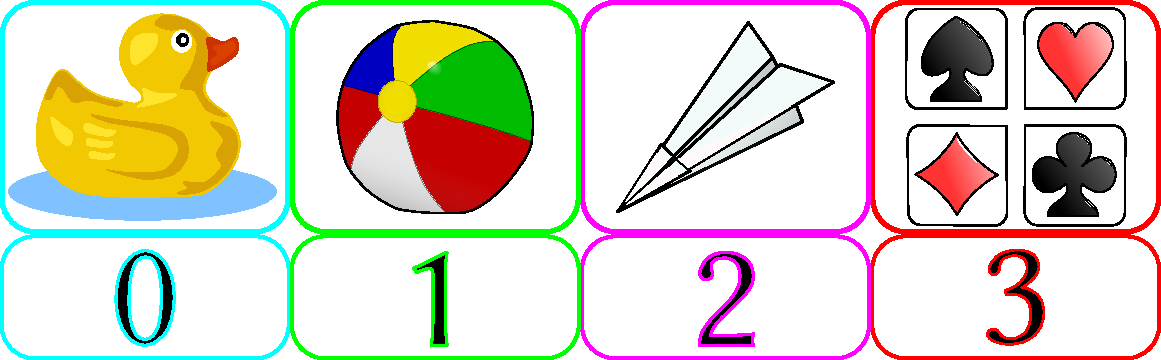
\includegraphics[scale=0.7]{images/liste.pdf} 

\end{center}
Nous pouvons utiliser tous les objets de la liste du troisième au cinquième, en utilisant deux points «~\verb+:+~» à l'intérieur des crochets:

\begin{Verbatim}[frame=single,rulecolor=\color{mbleu}, label=à taper]
>>> print(courses[2:5])
['céleri', 'confiture', 'sirop']
\end{Verbatim}

Utiliser «~\verb+[2:5]+~» est une autre manière de dire que nous sommes intéressés par les objets depuis l'index 2 jusqu'à l'index 5, mais sans l'inclure. Et, bien sûr, comme nous commençons à compter à 0, le 3\up{e} dans la liste est, en fait, le numéro 2 et le 5\up{e} est, en fait, le numéro 4. Les listes peuvent être utilisées pour conserver toutes sortes d'objets. Elles peuvent stocker des nombres:\\


\begin{Verbatim}[frame=single,rulecolor=\color{mbleu}, label=à taper]
>>> maliste = [ 1, 2, 5, 10, 20 ]
\end{Verbatim}

Des chaînes:

\begin{Verbatim}[frame=single,rulecolor=\color{mbleu}, label=à taper]
>>> maliste = [ 'a', 'bbb', 'ccccccc', 'ddddddddd' ]
\end{Verbatim}

Des mélanges de nombres et de chaînes:

\begin{Verbatim}[frame=single,rulecolor=\color{mbleu}, label=à taper]
>>> maliste = [1, 2, 'a', 'bbb']
>>> print(maliste)
[1, 2, 'a', 'bbb']
\end{Verbatim}


Et même des listes de listes:

\begin{Verbatim}[frame=single,rulecolor=\color{mbleu}, label=à taper]
>>> liste1 = [ 'a', 'b', 'c' ]
>>> liste2 = [ 1, 2, 3 ]
>>> maliste = [ liste1, liste2 ]
>>> print(maliste)
[['a', 'b', 'c'], [1, 2, 3]]
\end{Verbatim}

Dans l'exemple ci-dessus, une variable appelée «~\texttt{liste1}~» est créée avec trois lettres, «~\texttt{liste2}~» est créée avec trois nombres et «~\texttt{maliste}~» est créée en utilisant liste1 et liste2. 
Les choses peuvent devenir vraiment compliquées, vraiment rapidement, si vous créez des listes de listes de listes de listes de listes de listes... Mais, par chance, il n'y a généralement pas vraiment besoin de faire des choses  aussi compliquées en Python\footnote{Python n'est pas un langage de Shadock.}. Néanmoins il est utile de savoir que vous pouvez mettre toutes sortes d'objets dans une liste en Python.\\

\emph{Et pas seulement vos courses.}\\

\section*{Remplacer des objets}

Nous pouvons remplacer un objet dans une liste en fixant sa valeur de manière similaire à celle que nous utilisons pour assigner une valeur à une variable. Par exemple, nous pouvons changer le céleri en laitue en assignant une valeur en index 2:\\

\begin{Verbatim}[frame=single,rulecolor=\color{mbleu}, label=à taper]
>>> liste_de_courses[2] = "laitue"
>>> print(liste_de_courses)
['lait', 'fromage', 'laitue', 'confiture', 'sirop']
\end{Verbatim}

Revenons à mon histoire d'étiquette: rappelez-vous je vous parlais d'étiquette et de variable qui pointait vers un objet. Imaginons que nous soyons plusieurs à utiliser la même liste de course. Je peux demander à mon cousin \emph{Poche} de m'aider.

\begin{Verbatim}[frame=single,rulecolor=\color{mbleu}, label=à taper]
>>> liste_courses_poche=liste_de_courses
>>> liste_courses_poche[3]="moutarde"
>>> print(liste_de_courses)
['lait', 'fromage', 'laitue', 'moutarde', 'sirop']
\end{Verbatim}

Comme nous le voyons les modifications vues comme faites sur «~\texttt{liste\_courses\_poche}~» et de «~\texttt{liste\_de\_courses}~», ont eu lieu sur l'objet qui portait l'étiquette. Les variables pointent sur des objets mais ne sont pas les objets.

\section*{Ajouter plus d'objets...}

\index{append}Nous pouvons ajouter des objets à une liste en utilisant une méthode appelée «~\texttt{append\footnote{Le mot «~\emph{append}~» signifie ajouter en anglais, du verbe latin \emph{appendere} de \emph{ad} (à la suite) et \emph{pendere} (pendre).}}~».

Une méthode est une action qui dit à Python ce que nous voulons qu'il fasse. Nous parlerons des méthodes plus tard, mais pour le moment, pour ajouter un objet à notre liste de courses, nous pouvons faire comme suit:
%\begin{small}

\begin{Verbatim}[frame=single,rulecolor=\color{mbleu}, label=à taper]
>>> liste_de_courses.append('chocolat')
>>> print(liste_de_courses)
['lait', 'fromage', 'laitue', 'confiture', 'sirop', 'chocolat']
\end{Verbatim}

%\end{small}

\emph{Ce qui à défaut d'autre chose, est déjà une liste de courses améliorée.}\\

\section*{... Et enlever des objets}
\index{del}Nous pouvons retirer des objets d'une liste en utilisant la commande «~\texttt{del}~» (abréviation de \emph{delete\footnote{Le mot «~\emph{delete}~» signifier détruire ou effacer en anglais du participe passé \emph{deletus} du verbe latin \emph{delere} (détruire).}}).

Par exemple, pour retirer le 5\up{e} élément dans la liste (sirop):

\begin{Verbatim}[frame=single,rulecolor=\color{mbleu}, label=à taper]
>>> del liste_de_courses[5]
>>> print(liste_de_courses)
['lait', 'fromage', 'laitue', 'confiture', 'chocolat']
\end{Verbatim}


Rappelez-vous que les positions commencent à zéro, donc «~\texttt{liste\_de\_courses[4]}~» faisait en fait référence au cinquième élément.

\section*{Deux listes valent mieux qu'une}

Nous pouvons joindre des listes ensemble en les additionnant, comme si nous additionnions deux nombres:

\begin{Verbatim}[frame=single,rulecolor=\color{mbleu}, label=à taper]
>>> liste1 = [ 1, 2, 3 ]
>>> liste2 = [ 4, 5, 6 ]
>>> print(liste1 + liste2)
[1, 2, 3, 4, 5, 6]
\end{Verbatim}


Nous pouvons aussi additionner les deux listes et placer le résultat dans une troisième variable:

\begin{Verbatim}[frame=single,rulecolor=\color{mbleu}, label=à taper]
>>> liste1 = [ 1, 2, 3 ]
>>> liste2 = [ 4, 5, 6 ]
>>> liste3 = liste1 + liste2
>>> print(liste3)
[1, 2, 3, 4, 5, 6]
\end{Verbatim}

Et nous pouvons multiplier une liste de la même manière que nous avons multiplié une chaîne:

\begin{Verbatim}[frame=single,rulecolor=\color{mbleu}, label=à taper]
>>> liste1 = [ 1, 2 ]
>>> print(liste1 * 5)
[1, 2, 1, 2, 1, 2, 1, 2, 1, 2]
\end{Verbatim}

Dans l'exemple ci-dessus, multiplier liste1 par cinq est une autre manière de dire «~répéter liste1 cinq fois~». Malgré tout la division «~\texttt{/}~»  et la soustraction «~\texttt{-}~» ne fonctionnent pas sur les listes.
Ainsi nous aurons des erreurs quand nous essayerons les exemples suivants:

\begin{Verbatim}[frame=single,rulecolor=\color{red}, label=erreur]
>>> liste1 / 20
Traceback (most recent call last):
File "<stdin>", line 1, in <module>
TypeError: unsupported operand type(s) for /: 'list' and 'int'
\end{Verbatim}

ou:

\begin{Verbatim}[frame=single,rulecolor=\color{red}, label=erreur]
>>> liste1 - 20
Traceback (most recent call last):
File "<stdin>", line 1, in <module>
TypeError: unsupported operand type(s) for -: 'type' and 'int'
\end{Verbatim}

\emph{Vous aurez même des messages d'erreur sacrément moches.}

\section{N-uplets et listes\label{sec:nuplets}}
Un n-uplet (mentionné plus tôt) est un petit peu comme une liste mais plutôt que d'utiliser des crochets vous utilisez des parenthèses. Vous pouvez utiliser des n-uplets de manière semblable aux listes:

\begin{Verbatim}[frame=single,rulecolor=\color{mbleu}, label=à taper]
>>> t = (1, 2, 3)
>>> print(t[1])
2
\end{Verbatim}

La différence principale est que, contrairement aux listes, les n-uplets ne peuvent pas être changés une fois que vous les avez créés. Si vous essayez de remplacer une valeur comme vous l'avez fait plus tôt avec la liste, vous aurez un autre message d'erreur:

\begin{Verbatim}[frame=single,rulecolor=\color{red}, label=erreur]
>>> t[0] = 4
Traceback (most recent call last):
File "<stdin>", line 1, in ?
TypeError: 'tuple' object does not support item assignment
\end{Verbatim}

Cela ne signifie pas que vous ne pouvez pas changer la variable qui pointe vers le n-uplet pour la faire pointer vers quelque chose d'autre. Par exemple, ce code fonctionnera bien:

\begin{Verbatim}[frame=single,rulecolor=\color{mbleu}, label=à taper]
>>> mavar = (1, 2, 3)
>>> mavar = [ 'Une', 'liste', 'de', 'chaînes.' ]
\end{Verbatim}

D'abord nous avons créé une variable «~\texttt{mavar}~» qui pointait sur un n-uplet de trois nombres. Puis nous avons changé mavar pour qu'elle pointe vers une liste de chaînes. Cela peut sembler bizarre au départ.

C'est un peu comme des coffres qui seraient fermés à clef avec des verrous. Chaque coffre a un verrou  (le nom de la variable) qui permet de l'ouvrir. Vous mettez quelque chose dans un coffre et vous l'identifiez avec votre cadenas. Puis finalement vous décidez d'utiliser le verrou  pour un autre coffre. 

Vous ne pouvez pas changer ce qu'il y a dans le coffre fermé. Mais vous pouvez toujours utiliser le verrou  sur un autre coffre.

Mais si vous pouvez ouvrir et fermer le coffre et ajouter et retirer ce qui vous plait; c'est une liste.

\section{À vous de jouer\label{PRATIQUE:8}}

Dans ce chapitre nous avons vu comment calculer des équations mathématiques simples en utilisant Python de manière interactive. Nous avons vu comment les parenthèses pouvaient changer les résultats d'une équation en contrôlant l'ordre des opérations qui étaient utilisées. Nous avons trouvé comment dire à Python de se rappeler de valeurs pour un usage futur, en utilisant des variables. En plus nous avons vu que Python utilise des «~chaînes~» pour stocker du texte et des n-uplets et des listes pour gérer plus d'un objet.

\subsection{Exercice 1}
Faites une liste de vos jouets favoris et nommez la «~jouets~». Faites une liste de vos plats préférés et nommez la «~plats~». Joignez ces deux listes nommez le résultat «~préférés~». Finalement affichez la variable «~préférés~»\footnote{Vous trouverez les réponses aux section «~À vous de jouer~» en annexe \ref{annexe:reponses}.}.

\subsection{Exercice 2}
Si vous avez trois boites qui contiennent vingt-cinq chocolats et dix sacs qui contiennent trente-deux bonbons, combien avez de friandises au total? 

Note: il s'agit de faire le calcul dans la console ou le shell Python

\subsection{Exercice 3}
Créez des variables pour votre prénom et votre nom. Maintenant créez une chaîne et utilisez des paramètres substituables pour votre y insérer votre prénom et votre nom.\\


Vous trouverez des pistes de réponses dans la \autoref{reponses:8}.
 \vfill
\begin{center}
 
\includegraphics[width=5cm]{images/Caduceus.pdf}
\end{center}
 \vfill

\newpage
\thispagestyle{empty}
\AddToShipoutPicture*{
 \put(0,0){
 \parbox[b][\paperheight]{\paperwidth}{
 \vfill
\begin{center}
 
\includegraphics[width=5cm]{images/ouroboros.pdf}
\end{center}
 \vfill
 }}}